% Manuel Lippert - Paul Schwanitz
% Physikalisches Praktikum

% Teilaufgabe 2

\section{Das invertierte Pendel}
\label{sec:invertPendel}
Das invertierte Pendel erzeugt eine \textit{nichtlinearer} Schwingung. Dabei besitzt das Pendel eine unten fest eingespannte Blattfeder mit Federkonstante $k$, welche über zwei horizontal in der Höhe $h$ und der Auslenkung $x_h$ angreifende Spiralfedern mit Federkonstante $k_s$ und der Auslenkung $\hat{x}$ angetrieben wird. Am oberen Ende der Blattfeder lässt sich ein Zusatzgewicht $M$ anbringen und der Winkel $\theta$ beschreibt den Winkel zwischen der Tangenten an der Pendelspitze und dem Lot. Weiterhin bezeichnet die Pendellänge $L$ die Länge zwischen dem Anfang und Ende der Blattfeder, welche vom Winkel $\theta$ abhängt (siehe Abb \ref{image:invertiertesPendel}).
\begin{center}
    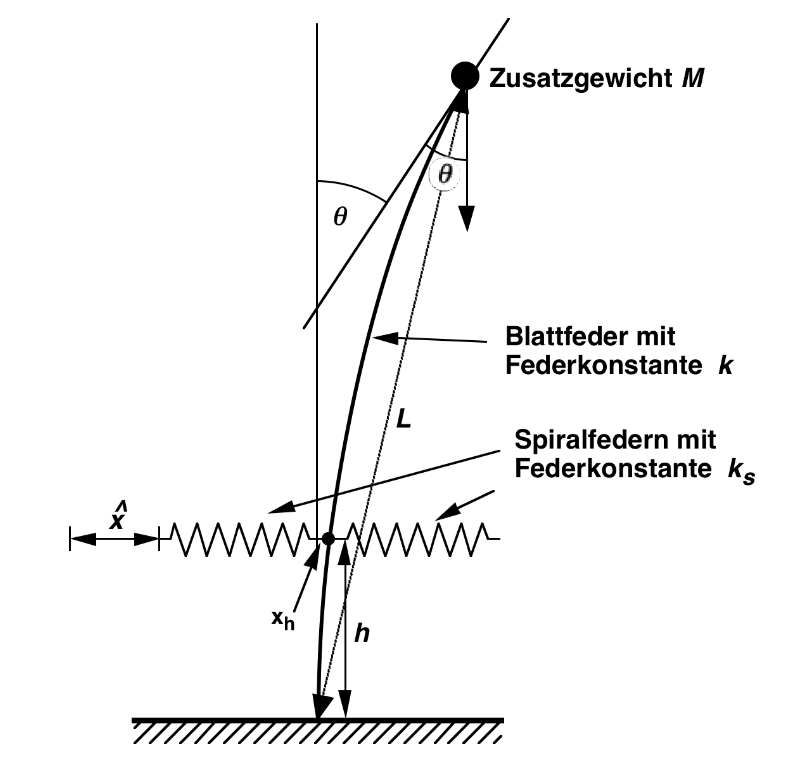
\includegraphics[scale=0.25]{Pendel/invertiertesPendel.png}
    \captionof{figure}{Skizze invertiertes Pendel \citep{Lueck}}
    \label{image:invertiertesPendel}
\end{center}
\subsection{Herleitung der Bewegungsgleichung}
\label{sub:bewegungsgleichung}
Die Bewegungsgleichung lässt sich über die wirkenden Drehmomente der Bauteile bestimmen:
\begin{gather*}
        \text{Pendel}~+~\text{Dämpfung}~+~\text{Blattfeder}~-~\text{Spiralfedern}~-~\text{Gewicht} = 0
\end{gather*}
\begin{gather}
    \Rightarrow [M(L(\theta))^2\ddot{\theta}]+[2\delta\dot{\theta}]+[k\theta]-[hk_s(x_h+\hat{x}\cos(\omega t))]-[MgL(\theta)\sin(\theta)]=0
\end{gather}
Dabei bezeichnet $\delta$ die Dämpfungskonstante und $g$ die Erdbeschleunigung.\\
Im Folgenden wird die Pendellänge $L$ als konstant angenommen, obwohl diese nicht konstant ist und von der Art der verwendeten Masse $M$ abhängt. Weiterhin wird die Auslenkung $x_h$ als vernachlässigbar klein angesehen und der Angriffswinkel der Spiralfedern wird als $\frac{\pi}{2}$ genähert, was bei genügend kleiner Höhe $h$ gegeben ist.
Daraus folgt die genäherte Form der Bewegungsgleichung:
\begin{gather}
    ML^2\ddot{\theta}+2\delta\dot{\theta}+k\theta-MgL(\theta)\sin(\theta)=hk_s\hat{x}\cos(\omega t)=T_0\cos(\omega t)
\end{gather}
Wobei $T_0$ als die Amplitude des periodisch angreifenden Drehmoments interpretiert werden muss. Hierbei ist noch zu erwähnen, dass durch die Näherungen die Lösung dieser Differentialgleichung nicht der tatsächlichen Trajektorien des Systems entsprechen, da diese stark von der Anfangsbedingung abhängen, dennoch ist eine globale Aussage über das Verhalten mit der genähreten Differentialgleichung möglich.\\
Zu den letzten beiden Termen lässt sich dann ein Potenzial definieren und durch Entwicklung des Cosinus für kleine Winkel $\theta$ (Kleinwinkelnäherung KWN) bis zur 2.Ordnung ergibt sich das Potenzial des \textit{Duffing-Oszillator} \citep{Lueck}.
\begin{gather}
    V(\theta) = \frac{1}{2}k\theta^2 + MgL(\cos(\theta)-1)\overset{\text{KWN}}{\approx}\frac{1}{2}(k-MgL)\theta^2 + \frac{1}{24}MgL\theta^4~,V(0)=0
\end{gather}

\subsection{Symmetriebrechung}
\label{sub:symbrechung}
Bei einer {kritischen Masse} $M_k=\frac{k}{gL}$ erfährt das System des Pendels einen Übergang von einem monostabilen System ($M<M_k$) in ein bistabiles System ($M>M_k$), dabei ist die Bewegung des Pendels in beiden Fällen Unterschiedlich und muss deshalb getrennt betrachtet werden. Bei diesem Übergang verändert sich die Struktur des Potenzial (siehe Abb \ref{image:potPendel}), wodurch nun zwei Lösungen für das System möglich sind. Das Auftreten von mehreren Lösungen in einem System wird dann auch \textit{\textbf{Symmetriebrechung}} genannt \citep{Lueck}.
\begin{center}
    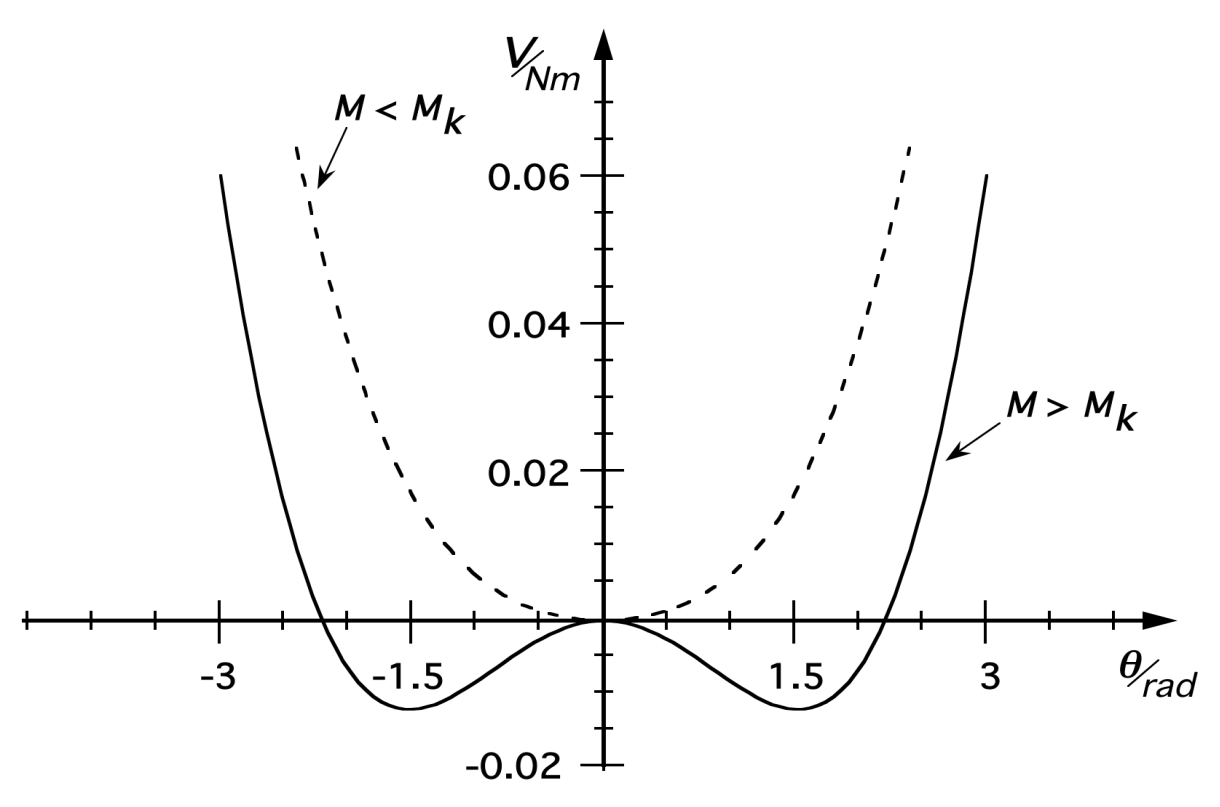
\includegraphics[scale = 0.2]{Pendel/PendelPotenzial.png}
    \captionof{figure}{Potenzialdarstellung für invertiertes Pendel \citep{Lueck}}
    \label{image:potPendel}
\end{center}

\subsection{Schwingungsdauer in Abhängigkeit der Masse}
\label{sub:schwingungsdauer}
Bei einem nichtlinearen Pendel hängt, im Gegensatz zu einem linearen Schwingungsvorgang, die Resonanzfrequenz $\omega_r$ von der Schwingungsamplitude $b$ ab $\Rightarrow \omega_r(b)$. Unverändert bleibt dennoch die Schwingungsamplitude $b(\omega)$ gegenüber der Resonanzkurve eines linearen Oszillators bei unterschiedlichen Anregungsfrequenzen $\omega$ \citep{Lueck}.
\begin{itemize}
    \item[1.] $M<M_k$ (Schwache Nichtlinearität)\\
    Pendel ist nach (\ref{sub:symbrechung}) monostabil. Der Vorgang lässt sich näherungsweise mit der Bewegungsgleichung eines Duffing-Oszillator nähern, wobei die Abhängigkeit der Resonanzfrequenz $\omega_r$ von der Amplitude $b$ berücksichtigt bleibt. Die Bewegungsgleichung lautet in diesem Fall:
    \begin{gather}
        \ddot{\theta} + 2\delta\dot{\theta} + \omega_0^2\theta + \gamma\theta^3 = f_a\cos(\omega t)
    \end{gather}
    Dabei bezeichnet $\gamma$ den Faktor der Nichtlinearität, $\omega_0$ die Resonanzfrequenz des Systems ohne Nichtlinearität ($\gamma=0$), $f_a$ die Anregungsamplitude mit Anregungsfrequenz $\omega$ und $\delta$ die Dämpfung.\\
    Durch Betrachtung des Verlaufs der Resonanzkurve in der Nähe von $\omega_0$ erhält man eine Gleichung dritter Ordnung für das Quadrat der Schwingungsamplitude $b$.
    \begin{gather}
        \left[\left((\omega^2-\omega_0^2) - \frac{3}{4}\gamma b^2\right)^2+(2\delta\omega)^2\right]b^2=f_a^2 %Angepasst an die Form in Wikipedia https://en.wikipedia.org/w/index.php?title=Duffing_equation&oldid=1031816809
        \label{eq:resonanzkurve}
    \end{gather}
    Diese Gleichung hat je nach Werten von $f_a, \gamma, \omega_0~\text{und}~\delta$ eine reelle oder zwei konjugierte komplexe Lösungen.
    Dabei ist es einfacher die Gleichung nach $\omega$ aufzulösen, wobei zur Vereinfachung $\omega_0=1$ angenommen wird. Damit wird (\ref{eq:resonanzkurve}) zu:
    \begin{gather}
        \left[\left((\omega^2-1) - \frac{3}{4}\gamma b^2\right)^2+(2\delta\omega)^2\right]b^2=f_a^2
    \end{gather}
    Mit der Lösung für $\omega$:
    \begin{gather}
        \omega^2_{1,2} = 1 - 2\delta^2 + \frac{3}{4}\gamma b^2 \pm \sqrt{\frac{f_a^2}{b^2}+ 4\delta^2\left[\delta^2 - \left(1 + \frac{3}{4}\gamma b^2\right)\right]}
    \end{gather}
    Bei hinreichender kleinen Dämpfung $\delta$ gibt es zwei verschiedene eingeschwungene Zustände, da die Lösung instabil wird (siehe Abb \ref{image:resonanzkurve}c)).
    \begin{center}
        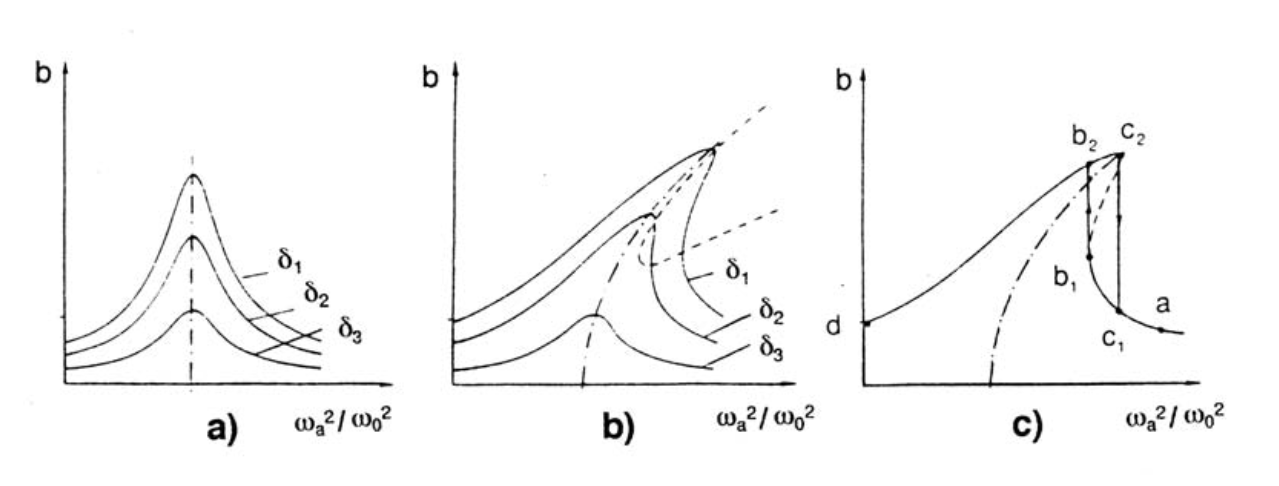
\includegraphics[scale=0.3]{Pendel/Resonanzkurve.png}
        \captionof{figure}{Resonanzkurven für eines Duffing-Oszillator \citep{Lueck}}
        \label{image:resonanzkurve}
        \captionof*{figure}{a) linearer ($\gamma=0$) b) nichtlinear c) Hysterese}
    \end{center}
    % https://www.ila.uni-stuttgart.de/nlvib/downloads/HB_NLvib_presentation.pdf, https://www.hindawi.com/journals/mpe/2011/248328/
    Die Schwingungsdauer $T$ hängt hierbei logarithmisch von der Amplitude $b$ ab mit dem Zusammenhang:
    \begin{gather}
        T = T_0 + T_1\log(b)
    \end{gather}
    Dies geht aus experimentellen Daten von \citep{Lueck} hervor, wobei $T_0$ und $T_1$ Näherungsparameter sind.
    \item[2.] $M>M_k$ (Starke Nichtlinearität)\\
    Das Pendel ist in diesem Fall nach (\ref{sub:symbrechung}) bistabil und besitzt zwei stabile Ruhelagen. Durch die Verringerung von großen Antriebsfrequenzen $\omega$ entstehen nach Ende des Einschwingverhaltens nacheinander subharmonische Schwingungen mit einer Periodenverdopplungskaskade ($T_n=2^nT=2^n\frac{2\pi}{\omega}$), obwohl sich das Pendel unterhalb einer kritischen Frequenz $\omega_k$ chaotisch verhält. Dieses Verhalten ist auch ein Beispiel für ein Bifurkationsszenario \citep{Lueck}.
\end{itemize}
\newpage
\subsection{Aufbau Pendel}
\label{sub:aufbauPendel}
\begin{center}
    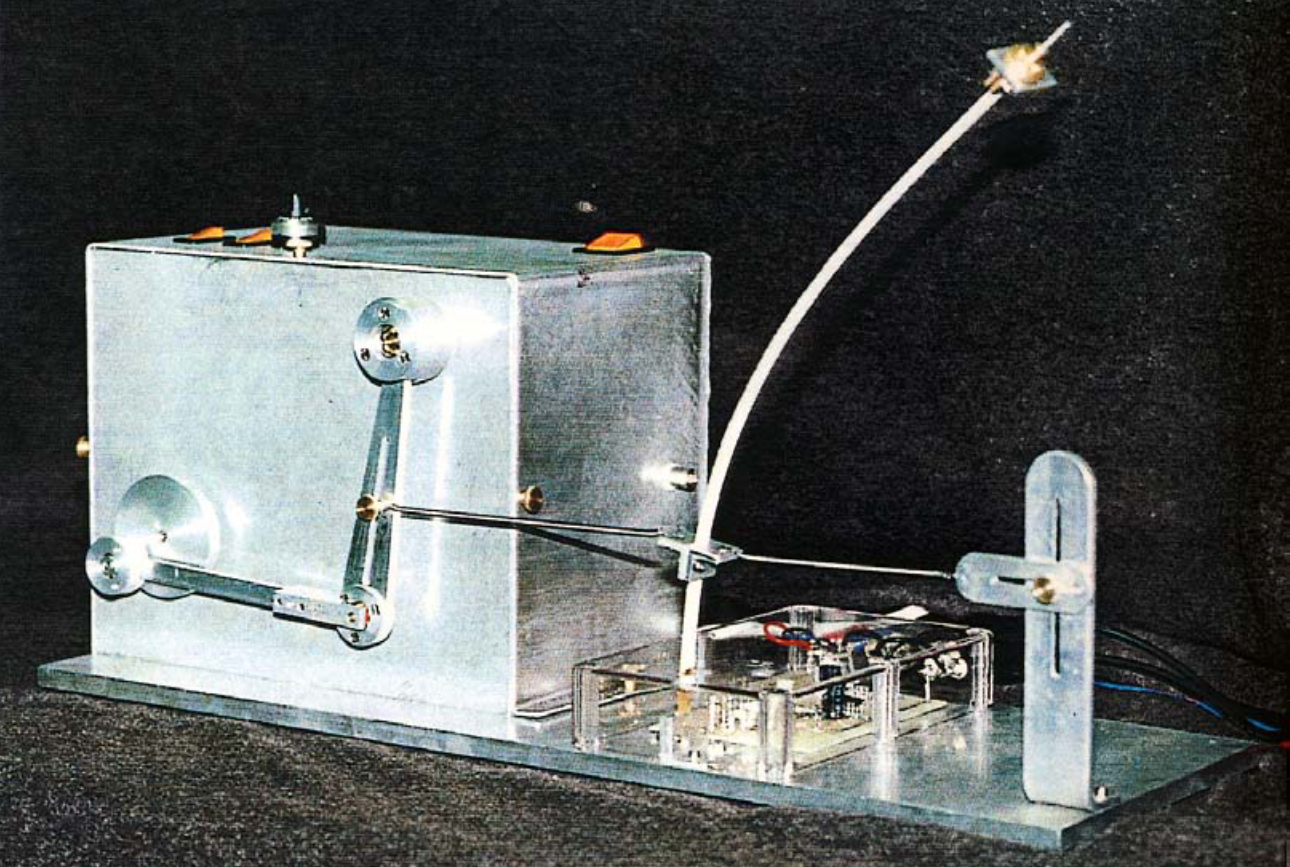
\includegraphics[scale=0.25]{Pendel/AufbauPendel.png}
    \captionof{figure}{Aufbau des invertierten Pendels \citep{Lueck}}
    \label{image:aufbauPendel}
\end{center}
Hierbei besteht das Pendel aus einer:
\begin{itemize}
    \item 5 mm starken Aluminium-Grundplatte
    \item 1 cm x 15 cm x 40 cm lange Blechstreifen aus einer Messing-Legierung mit hohem Kupferanteil, Dehnungsmessstreifen auf beiden Seiten (DMS, Widerstand abh. von der Dehnung) knapp oberhalb der Befestigung $\rightarrow$ Blattfeder
    \item Spiralfedern mit Federkonstante $k=027$ N/cm 
    \item Schrittmotor im Gehäuse mit 200 bzw. 400 Schritten (Halbschrittbereich)
    \item Multifunktionskarte Typs DAS 1602 der Firma Keithley (Taktimpulsgeber für Schrittmotoren)
\end{itemize}
Mit diesem Aufbau sind bis zu ca 5 Umdrehungen/s möglich, wobei die Antriebskraft durch das Verändern des Angriffspunktes der Spiralfeder am Übertragungshebel variierbar ist \citep{Lueck}.

\subsection*{Funktionsweise Differenzier-Schaltung}
Bei einer Differenzier-Schaltung wird nur die Änderung der Eingangsspannung zu einer Ausgangsspannung verarbeitet. Dabei wird ein Kondensator am Eingang in Reihe und ein Widerstand parallel zwischen Eingang und Ausgang des Operationsverstärker geschaltet. Durch den Kondensator fließt nur Strom, wenn sich die Eingangsspannung ändert, wobei die Ausgangsspannung proportional zur Änderungsgeschwindigkeit der Eingangsspannung ist. Durch den Operationsverstärker wird dann das Signal verstärkt, um dieses Signal besser über ein angeschlossenes Messgerät (z.B. Oszilloskop) betrachten zu können \citep{electronik}.

\begin{center}
    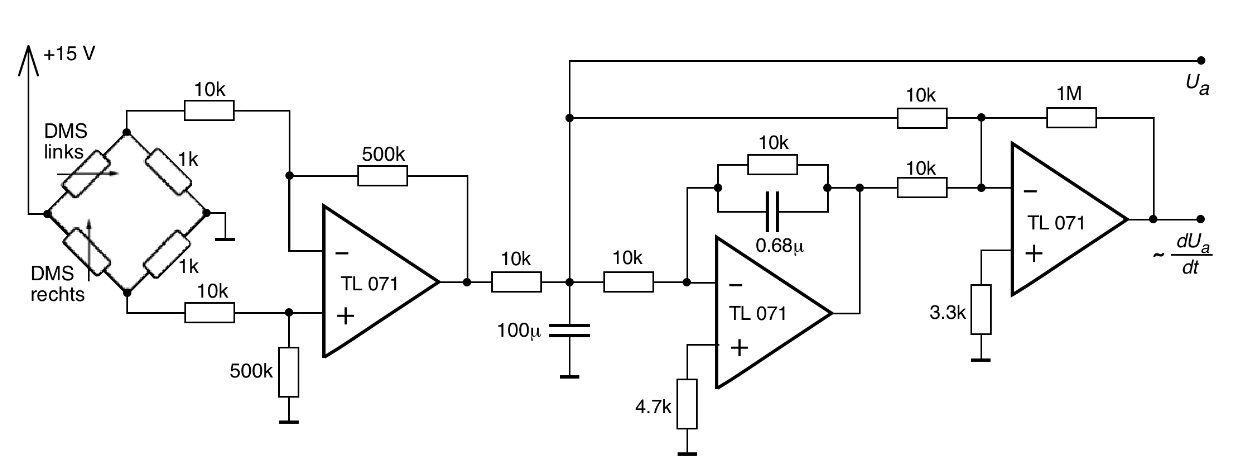
\includegraphics[scale=0.3]{Pendel/MessschaltungPendel.png}
    \captionof{figure}{Messschaltung des invertierten Pendels \citep{Lueck}}
    \label{image:schaltungPendel}
\end{center}
Für die Messschaltung (siehe Abb. \ref{image:schaltungPendel}) wird für eine höhere Genauigkeit zwei DMS in einer Brückenschaltung verschalten, um die Spannungsdifferenz von ihnen zu messen, wobei die Spannung dann proportional zur Pendelauslenkung $\theta$ ist. Für das Abgreifen der Geschwindigkeit als zweite Phasenraumvariable werden die Spannungen über eine Operationsverstärker-Schaltung differenziert. Die Spannungen werden dann einem im PC eingebauten Analog-Digital-Wandler-Karte gemessen, wobei die Messkarte über LABVIEW (Messprogramm) gesteuert wird \citep{Lueck}.